در فصول گذشته روش آزمون ...

\section{معرفی مطالعه‌ی موردی }
\label{section:caseDesign}
\begin{itemize}
\item خصوصیت ۱

\item خصوصیت ۲
\end{itemize}

\subsection{زیر بخش}
در فرآیندهای شناخته شده‌ی تولید نرم‌افزار (مانند \lr{RUP}) یکی از مهم‌ترین فرآورده‌های تحلیل سیستم، \glspl*{مورد کاربرد}\LTRfootnote{use cases} سیستم است. هر مورد کاربرد، در قالب متنی، نشان می‌دهد که رفتار سیستم در تعامل با محیط چگونه است. به عبارت دیگر موارد کاربرد توصیف‌های سطح بالای رفتاری سیستم هستند که به صورت غیر رسمی (ولی با درجات جزئیات متفاوت) بیان می‌شوند. در چهارچوب مورد بحث در این فصل فرض بر آن است که موارد کاربرد برای سیستم مورد نظر تهیه شده و موجود است. 

\subsubsection{تولید مدل رفتاری سیستم}
از آن‌جا که رفتار سیستم در قبال هر کنش محیط در مورد کاربرد مشخص شده است، می‌توان از آن مستقیماً برای تولید نمودارهای حالت استفاده نمود. در این تبدیل هر گام در شرح مورد کاربرد که توسط سیستم یا بر روی سیستم اعمال می‌شود، باعث حرکت آن از یک حالت به حالت دیگر خواهد شد. مطابق قرارداد، در ازای هر سناریوی اصلی حتماً یک ماشین مستقل طراحی می‌شود. هم‌چنین در صورتی که مدل‌سازی سناریوهای فرعی در همان نمودار سناریوی اصلی دشوار باشد می‌توان آن‌ها را نیز در ماشین‌های مستقلی مدل‌سازی نمود.

در مدلی که در این مرحله تولید می‌شود، نیازی به مشخص کردن کنش‌‌هایی که باعث حرکت بین حالت‌های مختلف ماشین می‌شوند وجود ندارد. در واقع نمودار به دست آمده در این مرحله، تنها به هدف مدل‌سازی نمای سطح بالای عملکرد سیستم و مجموعه‌ی حالت‌های آن طراحی می‌شود. مطابق قرارداد، مجموعه‌ی این نمودارهای حالت در یک \gls*{بسته‌}ی\LTRfootnote{package} یو‌ام‌ال به نام {\large\lr{\texttt{def::modeling::system}}} قرار خواهد گرفت.

\textbf{مثال. } نمودار حالت مربوط به سناریوی خرید (که پیش از این مطرح شد) در شکل \ref{fig:purchasePOS} رسم شده است. همان‌طور که مشاهده می‌شود، این سناریو از زمانی که یک مشتری کارت خود را به دستگاه نشان می‌دهد شروع شده و با توجه به نحوه‌ی اجرای سناریوهای اصلی و فرعی در یکی از سه نقطه‌ی پایانی متوقف می‌شود. در این نمونه‌ی خاص، با توجه به حجم نسبتاً پایین مدل تولید شده، سناریوهایی فرعی نیز در کنار سناریوی اصلی در یک ماشین مدل‌سازی شده‌اند.

\begin{figure}
    \begin{center}
    \begin{tabular}{| c |}
   	\hline
	\\
  	 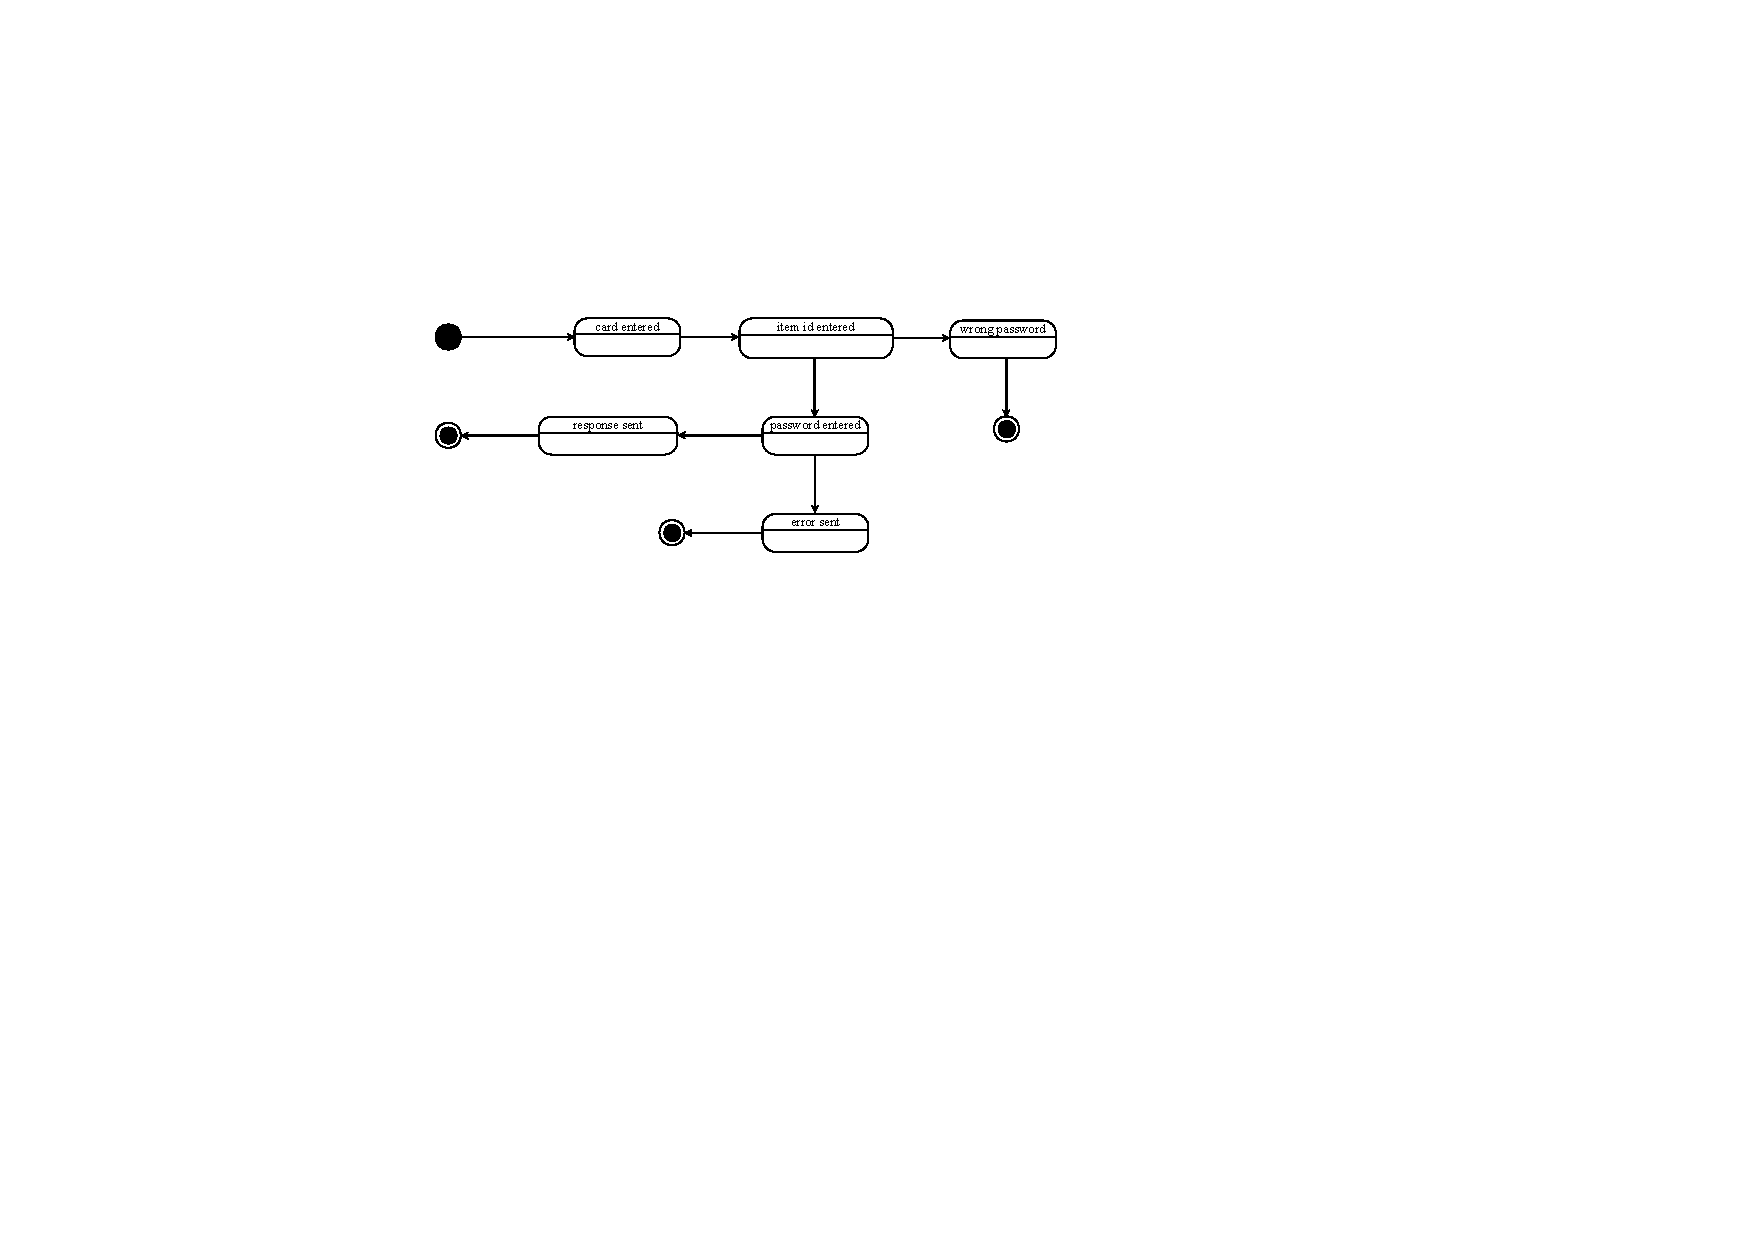
\includegraphics[width=12cm]{4-ProposedFramework/Figures/purchasePOS.pdf}
	\\
	\hline
  \end{tabular}
  \end{center}
   \caption{\label{fig:purchasePOS} ماشین‌حالت تولید شده برای رفتار پایانه فروشگاهی (سیستم) مثال}
\end{figure}

\subsubsection{تولید مدل رفتاری محیط}
آن‌چه که در ادامه‌ی این متن \emph{محیط عملکرد} و یا اختصاراً محیط نامیده می‌شود، به طور دقیق عبارت است از اکتورهایی که در یک مورد کاربرد با سیستم در ارتباطند. همان‌طور که پیش از این نیز گفته شد، برای حفظ هم‌خوانی ماشین‌های طراحی شده با مفهوم نمودار حالت یو‌ام‌ال هر نمودار از رفتار محیط باید شامل عملکرد \textbf{فقط} یک اکتور باشد. 

\textbf{مثال. } نمودارهای محیط برای دو اکتور مشتری و صندوق‌دار مثال مورد کاربرد خرید، در شکل \ref{fig:purchaseEnv} آمده است. همان‌طور که مشاهده می‌شود در هر نمودار تنها رفتار مربوط به همان اکتور ذکر شده است. 
\begin{figure}
    \begin{center}
    \begin{tabular}{| c |}
   	\hline
	\\
  	 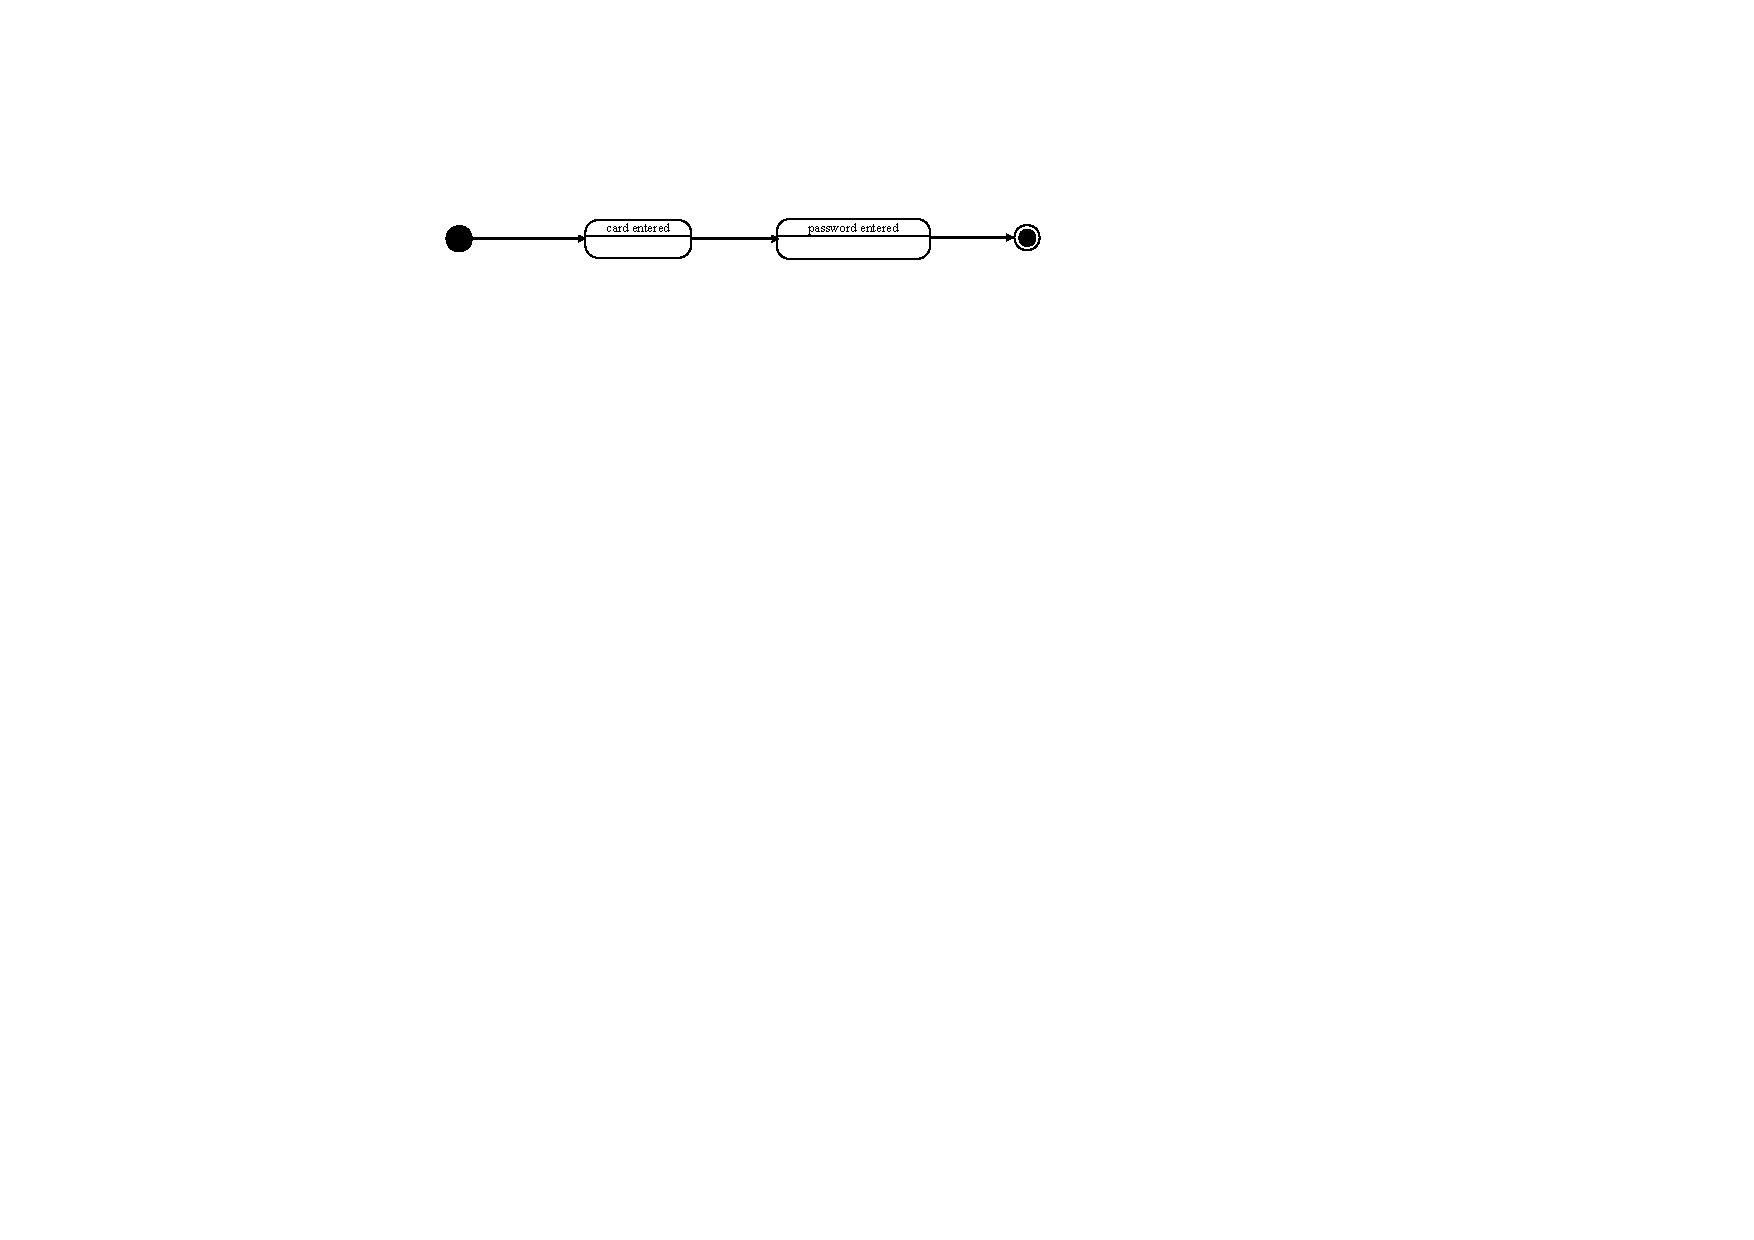
\includegraphics[width=12cm]{4-ProposedFramework/Figures/purchaseCust.pdf} \\
	(الف)\\ 
	\hline
	\\
 	 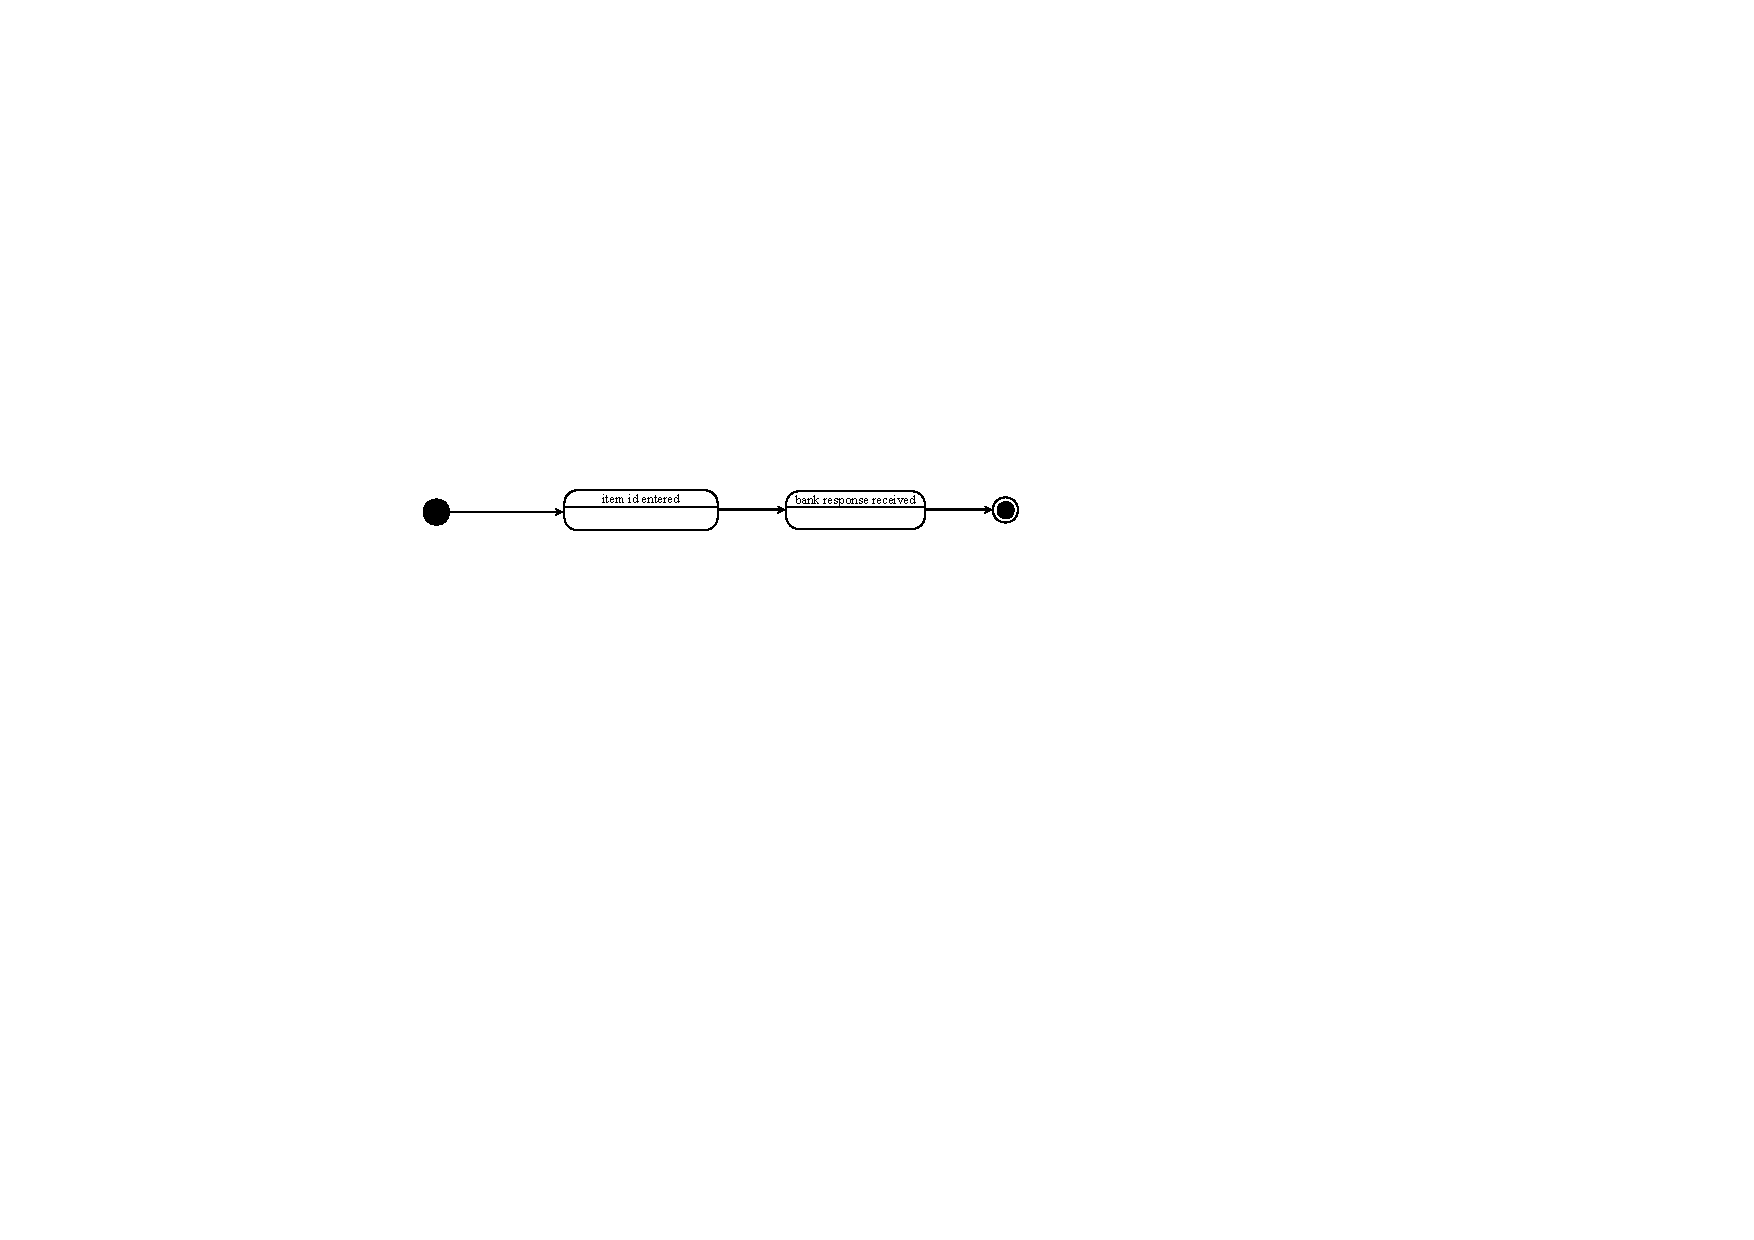
\includegraphics[width=12cm]{4-ProposedFramework/Figures/purchaseCash.pdf} \\
	\\	
	(ب)\\ 
	\hline
  \end{tabular}
  \end{center}
   \caption{\label{fig:purchaseEnv} ماشین‌حالت تولید شده برای دو اکتور محیطی در فرآیند خرید. (الف). مشتری و (ب) صندوق‌دار}
\end{figure}

اگرچه در مورد چگونگی تاثیر مدل‌های محیط بر رابطه‌ی مطابقت و الگوریتم تولید موارد آزمون در بخش بعد به تفصیل بحث خواهد شد، اما لازم است در این‌جا به مفهوم نمودارهای محیط توجه شود. توصیف محیط آزمون در واقع محدودکننده‌ی رفتار سیستم محسوب می‌شود. در مثال بالا در صورتی که مشتری هنگام وارد کردن رمز عبور همیشه رمز عبور صحیح را وارد نماید، با توجه به نمودار حالت مشتری سیستم هرگز وارد حالت \lr{``wrong password''} (در نمودار رفتار سیستم) نمی‌شود، بنابراین این مسیر هرگز اجرا نخواهد شد.

همانند آن‌چه در مورد نمودارهای سیستم ذکر شد، نمودارهای به دست آمده از محیط در این مرحله نیز کنش‌ها را مدل‌سازی نمی‌کنند. این نمودارها در بسته‌ی {\large\lr{\texttt{def::modeling::environment}}} قرار خواهند گرفت.
\subsubsection{مشخص کردن و تعریف گونه‌های داده‌ای}
اگرچه این بخش به توصیف مدل‌سازی رفتاری سیستم و محیط اختصاص دارد، اما باید توجه کرد که تکمیل مدل‌های رفتاری نمی‌تواند کاملاً مستقل از داده‌هایی که بین اجزای مدل مبادله می‌شوند، انجام شود. همان‌طور که پیش از این در فصل \ref{subsection:dataioco} اشاره شد،‌ تعیین رفتار در سیستم مبتنی بر داده، ممکن است مبتنی بر مقادیر داده‌ای آن باشد. برای مثال ممکن است سیستم بر اساس شرط‌هایی که روی متغیرهای خود قرار داده است، بین دو گذار متفاوت که از یک مکان ماشین نمادین خارج می‌شوند یکی را انتخاب نماید. همین رویه در مورد نمودارهای حالت به کار رفته برای توصیف در این چهارچوب وجود دارد. به همین منظور لازم است تا در خلال توصیف رفتاری، برخی خصوصیات پایه‌ای داده‌های سیستم نیز توصیف شوند.

مطابق قرارداد، در چهارچوب پیش‌رو هر مقدار داد‌ه‌ای لزوماً دارای گونه‌ای است که باید از پیش مشخص شده باشد. به همین منظور لازم است قبل از افزودن هر مقدار داده‌ای به توصیف‌ها، گونه‌ی آن مقدار تعریف شده باشد. یکی از منابع اصلی برای تشخیص گونه‌های موجود در یک توصیف، همان موارد کاربردی است که پیش از این نیز مورد استفاده قرار گرفته بود. دلیل این امر آن است که در متن موارد کاربرد، معمولاً توصیف داده‌های که در آن مورد کاربرد بین اکتورها رد و بدل می‌شود نهفته است. با استخراج این پارامترها از شرح موارد کاربرد موجود از یک سو و استفاده از دانش تیم پیاده‌سازی برنامه به عنوان یک منبع جانبی، از سوی دیگر می‌توان به مجموعه‌ای از گونه‌های داده‌ای رسید که باید مشخصاً در مدل‌سازی لحاظ شوند.

\textbf{مثال. }  در مثال فرآیند خرید می‌توان به راحتی پارامترهای داده‌ای زیر را از شرح موارد کاربرد استخراج نمود: 
\begin{itemize}
\item شناسه‌ی شناسایی کارت مشتری که به سیستم وارد می‌شود.
\item شناسه‌ی کالای مورد نظر که توسط صندوق‌دار به سیستم وارد می‌شود.
\item شماره‌ی رمز عبور مشتری که توسط خود او به سیستم داده می‌شود.
\item نتیجه‌ی خرید که خروجی پایانه‌ی فروش (سیستم) به مشتری و صندق‌دار (محیط) است.
\end{itemize}
در این مثال فرض می‌شود، اطلاعات خارجی (برای مثال دانش کسب شده از متن برنامه و یا از تیم پیاده‌سازی) نشان می‌دهد که کد شناسایی کارت، کد شناسایی محصول و شماره رمز کارت از نوع عدد طبیعی‌اند (که می‌توانند تا ۱۶ رقم طولانی باشند) و نتیجه‌ی خرید از نوع رشته‌های حرفی\LTRfootnote{string} است. هم‌چنین در مورد طراحی کارت فرض می‌شود که رمز صحیح هر کارت نیز (با همان گونه‌ای که رمز کارت نمایش داده می‌شود) نیز در کارت وجود دارد که در هنگام نشان دادن کارت به دستگاه خوانده می‌شود.

بعد از مشخص شدن گونه‌های داده‌ای، لازم است این گونه‌ها در زبان یوام‌ال تعریف شوند. این گونه‌ها باید همان گونه‌های داده‌ای تعبیه شده در توصیف زبان یو‌ام‌ال یا گسترشی از آن‌ها باشند. در صورتی که یک گونه به صورت گسترشی از یک گونه‌ی پیش‌فرض تعریف می‌شود، باید مجموعه‌ای از محدودیت‌ها را نیز تعریف کند که نشان‌دهنده‌ی تفاوت آن با گونه‌ی اصلی است. در چهارچوب پیشنهادی اجازه‌ی تعریف گونه‌های مستقل (یعنی گونه‌ای که از گونه‌ی دیگری گسترش نیافته است) وجود ندارد. گونه‌های داده‌ای نیز همانند بقیه‌ی اجزای مدل‌سازی این چهارچوب باید با استفاده از \gls*{کلیشه}‌ی\LTRfootnote{stereotype} \lr{‍‍``primitive''} از \gls*{عنصر}\LTRfootnote{element} کلاس یو‌ام‌ال، تعریف شده و در بسته‌ی {\large\lr{\texttt{primitives::datatypes}}} قرارگیرند.

\begin{figure}
    \begin{center}
    \begin{tabular}{| c |}
   	\hline
	\\
  	 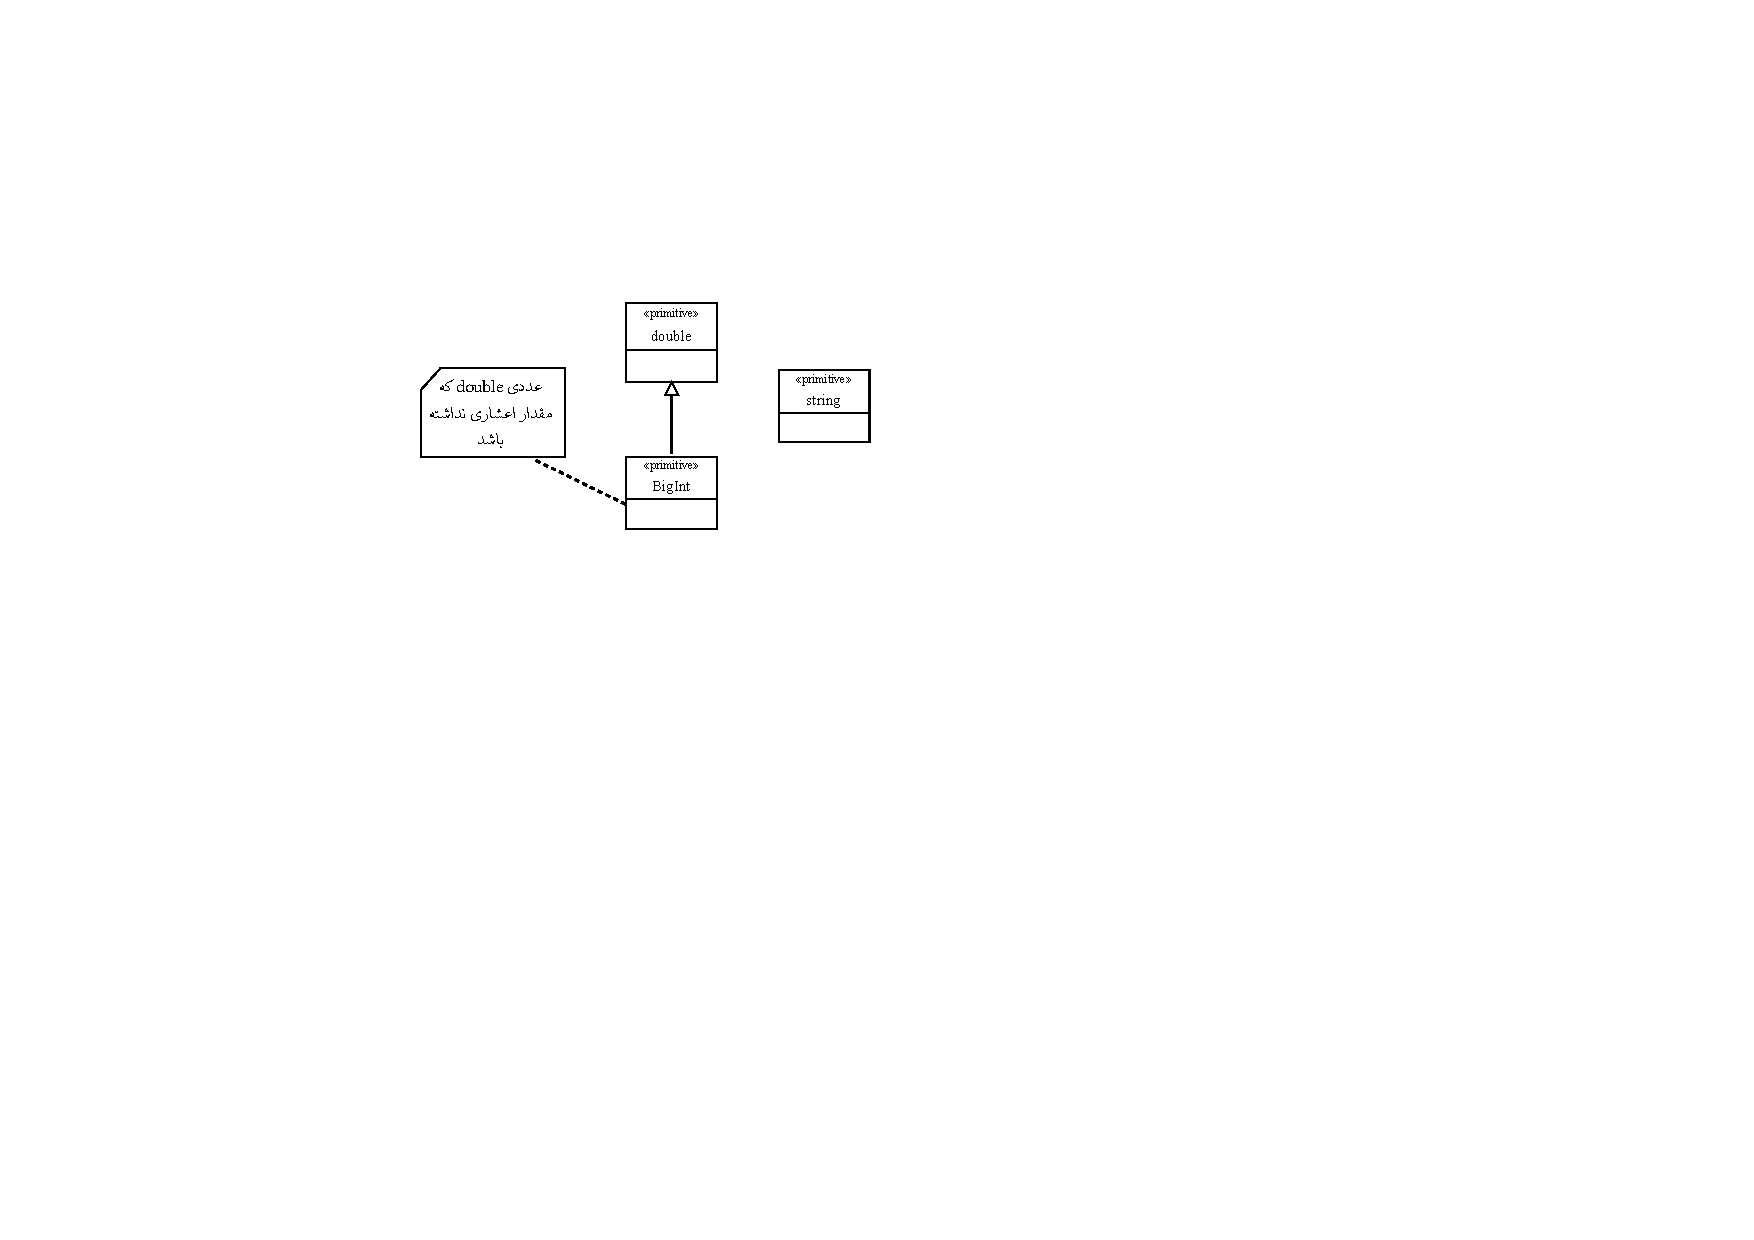
\includegraphics[width=8cm]{4-ProposedFramework/Figures/purchaseTypes.pdf} \\
	\\
	\hline
  \end{tabular}
  \end{center}
   \caption{\label{fig:purchaseTypes} مجموعه‌ی گونه‌های داده‌ای برای مثال فرآیند خرید}
\end{figure}

\textbf{مثال. } شکل \ref{fig:purchaseTypes} گونه‌های داده‌ای مثال خرید را نشان می‌دهد. در این شکل گونه‌های \lr{string} و \lr{double} گونه‌های تعبیه شده در خود زبان \lr{UML} هستند و \lr{BigInt} گونه‌ای گسترش‌یافته از \lr{double} است، با این محدودیت که اعضای آن نمی‌توانند اعشاری باشد (اما می‌تواند با استفاده از حجم اعداد \lr{double} اعداد بزرگ را نیز نمایش دهند).

\subsubsection{تعریف سیگنال‌های و پارامترهای آن‌ها}
تعریف سیگنال‌ها و پارامترهای آن‌ها با توجه به خروجی مرحله‌ی قبل بسیار آسان است، زیرا اولاً پارامترهای هر سیگنال در مرحله‌ی قبل معرفی شده و ثانیاً گونه‌ی داده‌ای آن نیز تعریف شده است. در نهایت، هر سیگنال ارتباطی لازم است توسط عنصر \lr{‍``signal''} که جزئی از ساختار زبان یوام‌ال است، طراحی شده و در بسته‌ی {\large\lr{\texttt{primitives::signals}}} قرار گیرد.

\textbf{مثال. } شکل \ref{fig:purchaseSignals} سیگنال‌های طراحی شده برای فرآیند خرید به همراه پارامترهای آن‌ها را نشان می‌دهد.
\begin{figure}
    \begin{center}
    \begin{tabular}{| c |}
   	\hline
	\\
  	 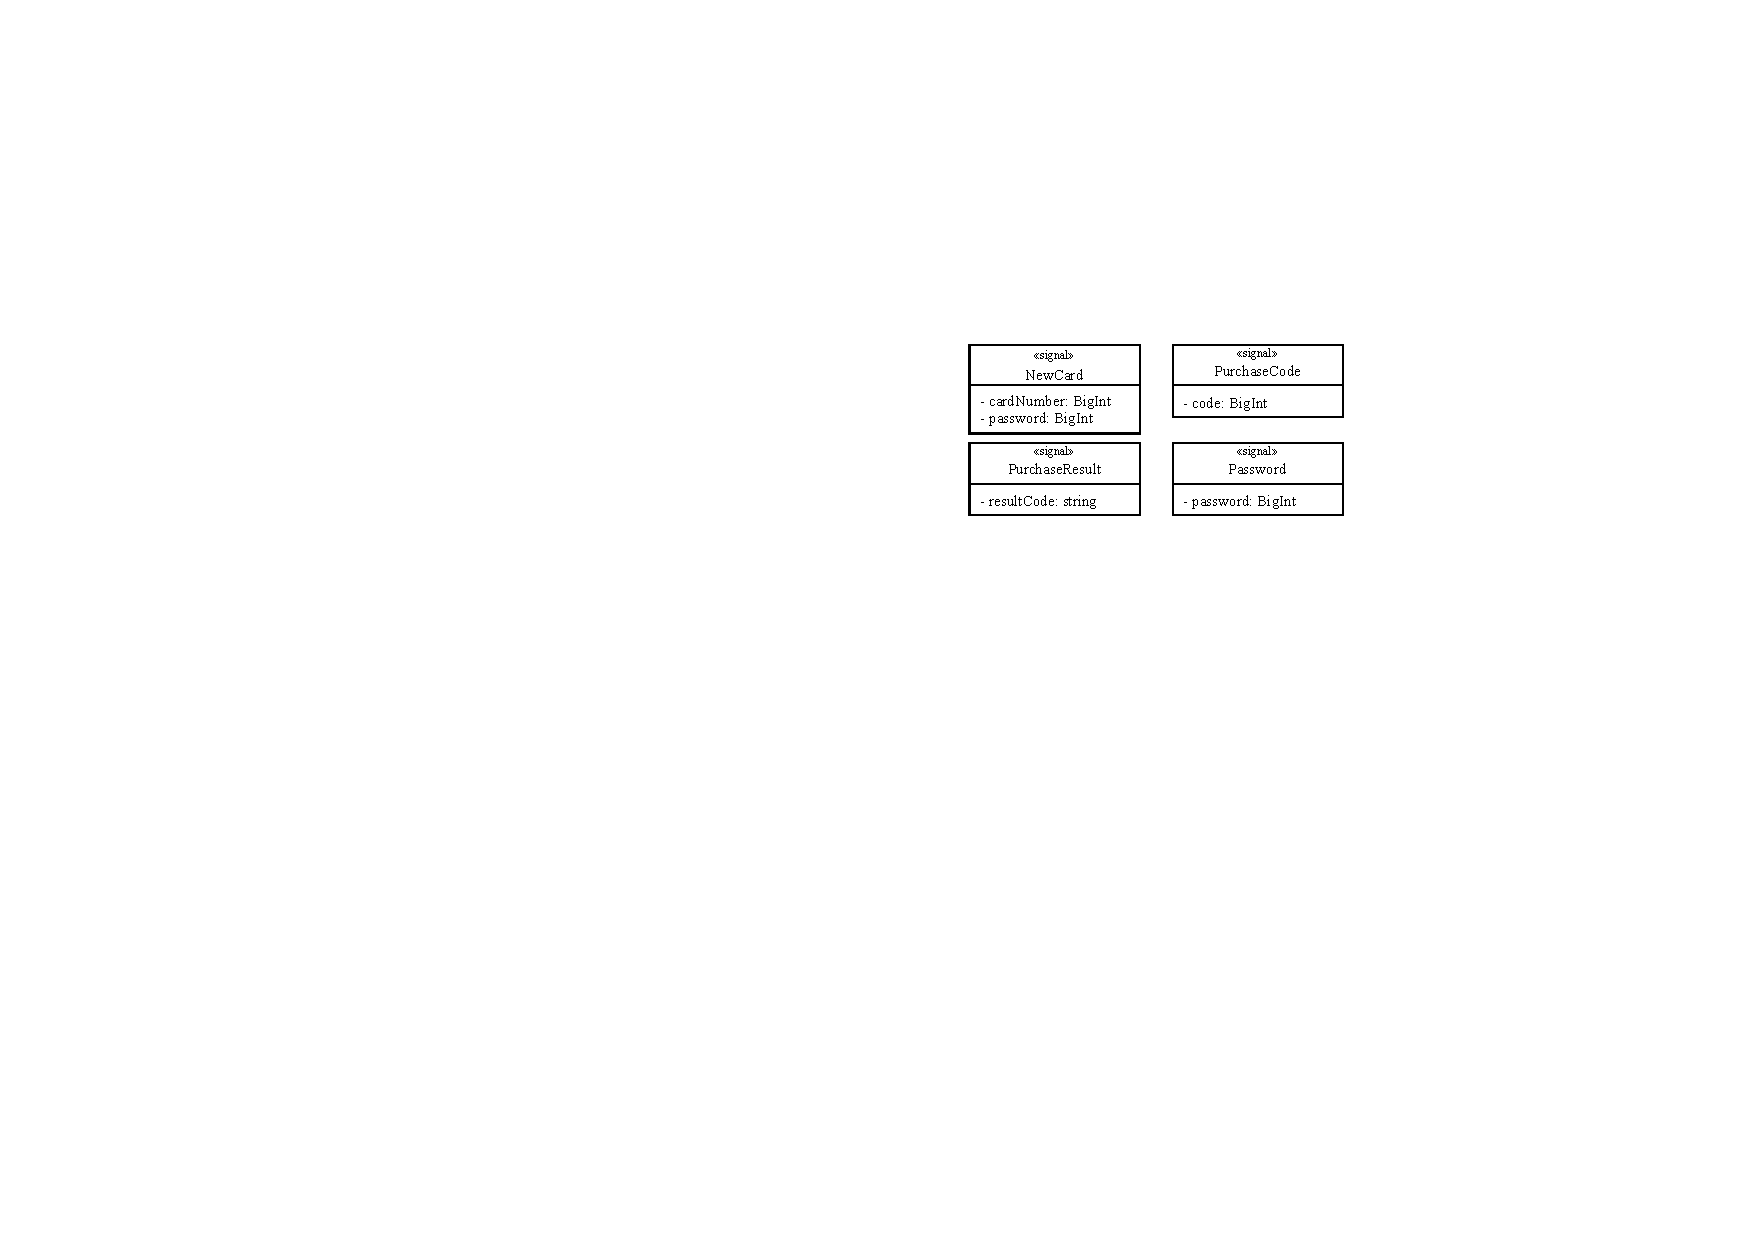
\includegraphics[width=8cm]{4-ProposedFramework/Figures/purchaseSignals.pdf} \\
	\\
	\hline
  \end{tabular}
  \end{center}
   \caption{\label{fig:purchaseSignals} مجموعه‌ی سیگنال‌ها برای مثال فرآیند خرید}
\end{figure}


\section{طراحی سیستم به روش ناهمگام}

\section{الگوها و سبک‌های طراحی}
\label{section:extracted_patterns}
پیش از این، نحو نمادگذاری مربوط به چهارچوب پیشنهادی این پژوهش تشریح شد. در این بخش، در مورد معنای هر یک از اجزای این نمادگذاری بحث خواهد شد. علاوه بر این، مطابقت معنایی این نمادگذاری را با مفاهیم آی‌اوکو مورد بررسی قرار داده و سپس الگوریتم جامعی برای تولید و اجرای یک‌پارچه‌ی آزمون‌هایی که با این نمادگذاری توصیف شده‌اند، ارائه خواهد شد.

\subsection{روشهای coordination }

\subsubsection{روش یک}
همان‌طور که پیش از این اشاره شد،‌ در چهارچوب پیشنهادی، توصیف‌های رفتاری چه برای سیستم و چه برای محیط در چندین نمودار حالت بیان می‌شود که هدف از آن کاهش پیچیدگی در طراحی مدل‌هاست. بنا به قرارداد، روش ترکیب این ماشین‌های حالت، روش میان‌گذاری است. به این معنی که 
\subsubsection{روش ۲}
همان‌طور که پیش از این اشاره شد، توصیف‌های رفتاری محیط نقش محدود‌کننده را در تولید موارد آزمون ایفا می‌کند. به عبارت دقیق‌تر با این‌که ممکن است موارد کاربرد مختلفی در یک سیستم پیاده شده باشد، ممکن است محیطی که سیستم در آن فعالیت می‌کند، تنها بخشی از این قابلیت‌ها را مورد استفاده قرار دهد. در این صورت با مدل‌سازی رفتار محیط می‌توان تنها درستی پیاده‌سازی این موارد کاربرد را آزمود. برای نمایش این مفهوم بر اساس نمادگذاری آی‌اوکو، لازم است رابطه‌ی مطابقت را بار دیگر به هدف بررسی مطابقت سیستم در حضور توصیف‌های محیط گسترش دهیم. در گام بعدی الگوریتم تولید موارد آزمون را نیز با توجه به این رابطه‌ی جدید، تعریف خواهیم نمود.



\subsection{سبک های طراحی}
سناریو‌های آزمون در چهارچوب پیشنهادی، تعیین کننده‌‌ی رو
با توجه به این تعاریف



\section{پیاده‌سازی}
\label{section:asyncImpl}
نحو و معنایی که برای توصیف چهارچوب پیشنهادی در این پژوهش مورد استفاده قرار گرفته است، در قالب یک مجموعه‌ی ابزار نیز پیاده‌سازی نیز شده 
